Graph clustering involves the task of dividing nodes into clusters, so that the edge density is higher within clusters as opposed to across clusters. Graph Clustering is a deeply studied problem as there are many use cases in biochemistry especially in clustering protein complexes. 

In this module we cluster similar solutions together to form some distinct types/methods/algorithms of solutions possible for the given problem.

The output from the above Similarity Measure module is considered as an edgelist in this module. The program files become the nodes and the similarity measure becomes the weights of the edge between them.

Using this graph, we start clustering. Idea is that nodes with edges whose similarity values are high will cluster together. 

The output of this module are clusters which contains program files.

\subsubsection{Implementation Details}
We use various clustering algorithms and compare their clusters to some human annotated clusters.
\paragraph{Louvain modularity}
    We use a method called Louvain modularity \cite{louvian} which is a greedy optimization method that appears to run in time O($n\log n$). In this method, first small communities are found by optimizing modularity locally on all nodes, then each small community is grouped into one node and the step is repeated.

    \textit{Observation:} Nodes within Clusters sometimes do not have high edge weights, while one node will be highly connected to everything the other nodes are not so strongly connected to each other node. 
    \textit{Possible explanation:} Since similarity values are calculated based on isomorphism which is NP-complete, the values for some pair of nodes might actually be high but since it cannot be found out in the stipulated time interval, the values are given zero. While clustering, if the neighbours of the nodes are highly similar then it is also highly likely that the node is similar to the rest of the others.
    
    For eg:
            For example there are 4 nodes 1,2,3 \& 4 if 1,2,3 are highly similar and 3,4 are also highly similar but the values for 1,4 and 2,4 are zero, it is highly possible that 1,4 and 2,4 are actually similar but the sub graph isomorphism could not find a solution within the given interval.
    
    \textit{Solution:} Add other parameters to include in similarity measurement. 
    
    
        \begin{figure}[H]
            \centering
                \centering
                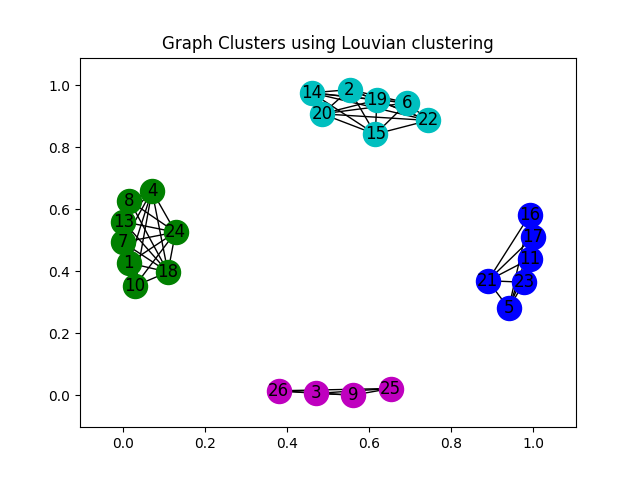
\includegraphics[scale=0.5]{Images/cluster_louvian_1.png}
                \caption{Louvian Clustering}
        \end{figure}
    
\paragraph{IPCA Clustering}
    Each point’s measure property can be transformed as the influence power against its neighbor points.\cite{ipca} If one point’s measure is larger, it would have more
influence power to attract its neighbor points, and its neighbors would have a trend to be absorbed by this point.

    \textit{Observation:} Within clusters, the similarity is high but same nodes are found in multiple clusters

        \begin{figure}[H]
            \centering
                \centering
                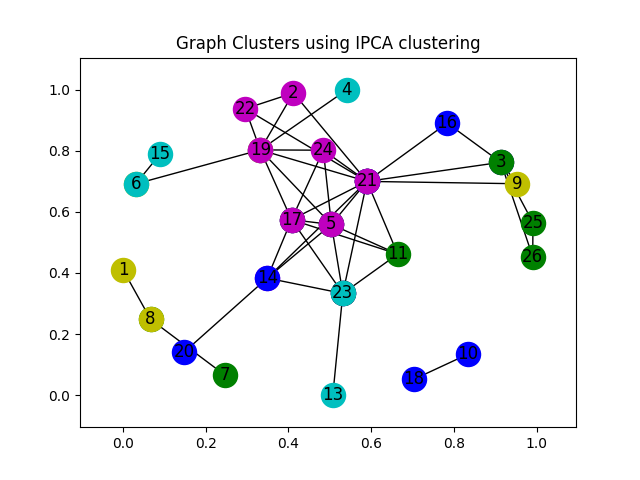
\includegraphics[scale=0.5]{Images/cluster_IPCA_1.png}
                \caption{IPCA Clustering}
        \end{figure}


%#TODO Put graphs images

